\documentclass[final]{siamltex}
%test change
\usepackage{cite}
\usepackage{graphicx,bbm,pstricks,soul}
\usepackage{pifont}
\usepackage{bbm,algorithmic,mdframed,placeins,multirow,booktabs,subfigure}
\usepackage[ruled,vlined,linesnumbered]{algorithm2e}
\usepackage{tikz,hhline}
\usepackage{tabularx}
\newcolumntype{L}[1]{>{\raggedright\let\newline\\\arraybackslash\hspace{0pt}}m{#1}}
\newcolumntype{C}[1]{>{\centering\let\newline\\\arraybackslash\hspace{0pt}}m{#1}}
\newcolumntype{R}[1]{>{\raggedleft\let\newline\\arraybackslash\hspace{0pt}}m{#1}}

\setlength{\parindent}{0in}
\usepackage{amsmath,amsfonts,amsbsy,amssymb}
\newcommand{\RARR}[3]{#1
  \;\displaystyle\mathop{\displaystyle\longrightarrow}^{#3}\; #2}
\newcommand{\RARRlong}[3]{#1
  \;\displaystyle\mathop{-\!\!\!-\!\!\!-\!\!\!-\!\!\!-\!\!\!\!\displaystyle
  \longrightarrow}^{#3}\; #2}
\newcommand{\LARR}[3]{#1
  \;\displaystyle\mathop{\displaystyle\longleftarrow}^{#3}\; #2}
\newcommand{\LRARR}[4]{{\mbox{ \raise 0.4 mm \hbox{$#1$}}} \;
  \mathop{\stackrel{\displaystyle\longrightarrow}\longleftarrow}^{#3}_{#4}
  \; {\mbox{\raise 0.4 mm\hbox{$#2$}}}}
\newcommand{\bX}{{\bf X}}
\newcommand{\vecx}{{\mathbf x}}
\newcommand{\vecy}{{\mathbf y}}
\newcommand{\vecz}{{\mathbf z}}
\newcommand{\vecq}{{\mathbf q}}
\newcommand{\bs}{{\mathbf s}}
\newcommand{\vecr}{{\mathbf r}}
\newcommand{\vecX}{{\mathbf X}}
\newcommand{\vecv}{{\mathbf v}}
\newcommand{\tick}{\ding{52}}
\newcommand{\cross}{\ding{54}}
\newcommand{\vecn}{{\mathbf n}}
\newcommand{\vecp}{{\mathbf p}}
\newcommand{\cT}{{\mathcal T}}
\newcommand{\dt}{{\mbox{d}t}}
\newcommand{\dx}{{\mbox{d} \vecx}}
\newcommand{\boldnu}{{\boldsymbol \nu}}
\newcommand{\er}{{\mathbb R}}
\renewcommand{\div}{{\rm div}}
\newcommand{\bnu}{{\bf \nu}}
\newcommand{\divergence}{\mathop{\mbox{div}}}
\renewcommand{\P}{\mathbb{P}}
\newcommand{\FP}{P_{\rm{FP}}}
\newcommand{\ME}{P_{\rm{ME}}}
\newcommand{\MEs}{P_{\rm{ME}_{S}}}
\newcommand{\D}{\mathcal{D}}
\newcommand{\G}{\mathcal{G}}
\newcommand{\N}{\mathcal{N}}
\newcommand{\X}{{\mathbf X}}
\newcommand{\Y}{{\mathbf Y}}
\newcommand{\W}{{\mathbf W}}
\newcommand{\data}{D}
\newcommand{\neff}{n_{\text{eff}}}
\newcommand{\E}{{\mathbb E}}
\renewcommand{\b}[1]{{\bf #1}}
\newcommand{\edit}[1]{{\color{red} #1}} 
\DeclareMathOperator*{\argmin}{arg\,min}
\DeclareMathOperator*{\argmax}{arg\,max}

\newcommand{\picturesAB}[6]{
\centerline{
\hskip #4
\raise #3 \hbox{\raise 0.9mm \hbox{(a)}}
\hskip #5
\epsfig{file=#1,height=#3}
\hskip #6
\raise #3 \hbox{\raise 0.9mm \hbox{(b)}}
\hskip #5
\epsfig{file=#2,height=#3}
}}
\newcommand{\picturesCD}[6]{
\centerline{
\hskip #4
\raise #3 \hbox{\raise 0.9mm \hbox{(c)}}
\hskip #5
\epsfig{file=#1,height=#3}
\hskip #6
\raise #3 \hbox{\raise 0.9mm \hbox{(d)}}
\hskip #5
\epsfig{file=#2,height=#3}
}}

\makeatletter  
\newcommand{\xleftrightarrows}[2][]{\mathrel{%  
 \raise.40ex\hbox{$  
       \ext@arrow 3095\leftarrowfill@{\phantom{#1}}{#2}$}%  
 \setbox0=\hbox{$\ext@arrow 0359\rightarrowfill@{#1}{\phantom{#2}}$}%  
 \kern-\wd0 \lower.4ex\box0}}  
 
\newcommand{\xrightleftarrows}[2][]{\mathrel{%  
 \raise.40ex\hbox{$\ext@arrow 3095\rightarrowfill@{\phantom{#1}}{#2}$}%  
 \setbox0=\hbox{$\ext@arrow 0359\leftarrowfill@{#1}{\phantom{#2}}$}%  
 \kern-\wd0 \lower.4ex\box0}}  
 
\def\leftrightarrowfill@{%
 \arrowfill@\leftarrow\relbar\rightarrow%
 }
\newcommand*{\centerfloat}{%
  \parindent \z@
  \leftskip \z@ \@plus 1fil \@minus \textwidth
  \rightskip\leftskip
  \parfillskip \z@skip}
\makeatother
\makeatother 

\newcommand\irregularcircle[2]{% radius, irregularity
  \pgfextra {\pgfmathsetmacro\len{(#1)+rand*(#2)}}
  +(0:\len pt)
  \foreach \a in {10,20,...,350}{
    \pgfextra {\pgfmathsetmacro\len{(#1)+rand*(#2)}}
    -- +(\a:\len pt)
  } -- cycle
}

\newcommand{\into}{\operatornamewithlimits{\longrightarrow}}
\newtheorem{dfn}{Definition}[section]

\newcommand{\ltri}{%
\,\resizebox{!}{0.25\baselineskip}{%
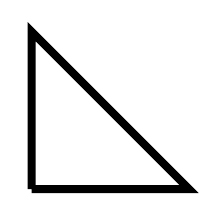
\begin{tikzpicture}%
\draw[line width=1mm](0,0) -- (0,2) -- (2,0)  -- (0,0);
\end{tikzpicture}%  
}\xspace%
}%

\newcommand{\smallltri}{%
\,\resizebox{!}{0.15\baselineskip}{%
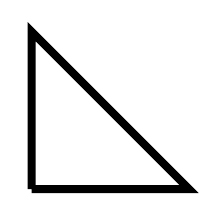
\begin{tikzpicture}%
\draw[line width=1mm](0,0) -- (0,2) -- (2,0)  -- (0,0);
\end{tikzpicture}%  
}\xspace%
}%

\author{Simon L. Cotter\thanks{School of
    Mathematics, University of Manchester, Manchester, UK. e:
    simon.cotter@manchester.ac.uk. SLC is grateful for EPSRC First
    grant award EP/L023393/1. SLC would like to thank the Isaac Newton
    Institute for Mathematical Sciences for support and hospitality
    during the programme ``Uncertainty quantification for complex systems: theory and methodologies'' when work on this paper was undertaken. This work was supported by:
EPSRC grant number EP/K032208/1.} \and Ioannis
G. Kevrekidis\thanks{Chemical and Biomolecular Engineering \& Applied
  Mathematics and Statistics, Johns Hopkins University, Baltimore, MD
  21218. The work of IGK was partially supported by the US National
  Science Foundation, by the US AFOSR, and by DARPA.} \and Paul
  Russell\thanks{School of
    Mathematics, University of Manchester, Manchester, UK.}}

\title{Multiscale Methods for Stochastic Chemical Reaction
  Networks:\\Supplementary material}
\begin{document}
\maketitle
\stepcounter{section}
\def\thesection{\alph{section}}
In this supplementary material, we discuss some recent advances in multiscale methods
for stochastic reaction networks. Inverse problems arising in this
area often lead to complex posterior
distributions, which traditional MCMC methods can struggle to sample
from.

We consider chemical reaction networks of $N_s$ chemical species $\{S_j\}_{j=1}^{N_s}$,
with population numbers given by $X(t) = [X_1(t), X_2(t), \ldots, X_{N_s}(t)]^\top \in
\mathbb{N}_0^{N_s}$ reacting in a small reactor, through $N_r$ different reaction
channels. When population numbers of one or more of the chemical
species in the reactor is small, as is the case with chemical
reactions occurring within living cells, the sporadic and discrete way
in which reactions occur can not be well modelled by deterministic
continuous models, such as ODEs. In such a situation, we may wish to
model the dynamics through a discrete stochastic model, such as a
continuous time Markov chain.

For each reaction $R_j$, for $j = 1,2,\ldots N_r$, there is a
propensity or hazard function $\alpha_j(X(t))$ which indicates how
likely that reaction is to fire, defined by
\[\alpha_j(X(t)) = \lim_{dt \to 0} \mathbb{P}(\text{Reaction $R_j$ in
    the time interval  } \quad s \in [t, t+ dt] ).\] If a system
satisfies what is called \emph{mass action kinetics}, then the form of
the function $\alpha_j$ is determined, up to a rate constant, by the
reactants involved in that reaction:
\begin{equation}\label{eq:MAK}
\alpha_j(X) = k_j \prod_{m=1}^{N_s} \prod_{n=0}^{\nu_{j,m} -1} (X_m - n),
\end{equation}
where $\nu_{j,m}$ is the $m$th component of the stoichiometric vector
$\nu_j$, $X_m$ is the $m$th component of the state vector $X$, and the
$k_j$ are rate constants.

Following each reaction $R_j$ there is an instantaneous change in the
current state, as the reactants of the reaction are consumed, and the
products produced. This is modelled by a change in the state vector
$X(t) = X(t) + \nu_j$ where $\nu_j$ is that stoichiometric vector for
reaction $R_j$.

The model can be represented as the following expression involving
$N_r$ different unit rate Poisson
processes\cite{anderson2011continuous} $Y_j$, given by:
\begin{equation}\label{eq:RTC}
X(t) = X(0) + \sum_{j=1}^{N_r} \nu_j \int_0^t \alpha_j(X(s)) ds.
\end{equation}

The master equation for this model is only solvable in certain
situations, for example monomolecular networks\cite{jahnke2007solving}, or for
steady-state solutions for weakly reversible deficiency
zero networks\cite{anderson2010product,anderson2016product}. Trajectories for this system can be
sampled exactly, for instance using the Gillespie SSA\cite{gillespie1977exact}, or
its variants\cite{gillespie2007stochastic,cao2004efficient,anderson2007modified}. However, if the system is stiff, i.e. there
are some reactions which are firing many times on a timescale for
which others are unlikely to fire at all, then trajectories can become
prohibitively expensive to simulate, since these methods simulate
every single reaction event with the same cost. In such a system, one
might employ multiscale methods in order to approximate trajectories
at a lower cost than the exact algorithms.

One common approach is to invoke the quasi-equilibrium approximation
QEA. This approximation makes the assumption that fast reactions
enter quasi-equilibrium on a timescale which is negligible with
respect to the timescale on which the slow dynamics in the system are
evolving. This amounts to taking the asymptotic limit that the
propensities of the ``slow'' reaction channels are equal to zero. This
allows us to sample approximate trajectories of the slow reactions
without the need to compute many fast reaction events.

This approach can work well when there is a large timescale gap
between the fast and slow reactions in a system, but where the
timescale gap is less pronounced, it can lead to significant
errors\cite{cotter2016error}. Another approach is the
constrained multiscale algorithm (CMA)\cite{cotter2011constrained,cotter2016constrained}, based in part on the
equation-free approach to multiscale computations\cite{kevrekidis2003equation,erban2006gene}. This approach also assumes quasi-equilibrium in the
system, but takes into account the effect that the slow reactions can
have on the invariant distribution of the fast variables in the
system. For a more detailed description of this method, please refer
to the literature\cite{cotter2016constrained}.

Multiscale methods are not only of use when forward evaluations of the
dynamics are costly, but can also be of use where we attempt to solve
an inverse problem where the fast variables are unobservable. One
approach in this situation would be to integrate over all possible
trajectories of the fast variables, but this would almost always be
prohibitively expensive. Another approach would be to use an
appropriate multiscale approximation, so that the effective dynamics
of the slow variables can be approximate without the need to consider
the rapid fluctuations of the fast variables in the system.

\subsection{Likelihoods arising from stochastic reaction networks}
Suppose that we are able to exactly observe the number of molecules of
each chemical species in a system which satisfies mass action
kinetics, and which can be well approximated by
\eqref{eq:RTC}. Suppose that we wish to be able to infer the value of
the rate constants of each reaction from these observations. Even with no observational noise, since the dynamics
of the system are stochastic, this still leads to a Bayesian inverse
problem where we can only infer a joint probability distributions on the
reaction parameters.

Suppose that we are in state $X(t) = X_0$. There are two independent
univariate random variables which decide when and what the next
reaction in the system is. There is the $j$th waiting time $\tau_j$ to the
next reaction, which is given by an exponential random variable
\[\tau_j \sim \exp \left ( \frac{1}{\alpha_0(X(t))} \right ),\]
where $\alpha_0(X(t)) =\sum_{i}^{N_r} \alpha_i(X(t))$ is the total
propensity in the system. The second is a multinomial random variable $r_j$
which dictates which reaction has occurred during the $j$th reaction,
which takes the value
$i \in \{1,2,\ldots,N_r\}$ with probability
\[\mathbb{P}(r_j = i) = \frac{\alpha_i(X(t))}{\alpha_0(X(t))}.\]
As such, in order to compute the likelihood of a particular trajectory
given a possible realisation of the reaction parameters, it is
sufficient to have access to the total time spent in each state, and
the frequency of each reaction which led to leaving each state.

From this formulation, we see that the random variables $(\tau_j, r_j)$ only depend on the states $\mathbf{X}(t_{j-1})$ and so are Markovian. This conditional independence means that we can group events together by what state the system was in when the event happened. We define two new random variables which depend on a state $\mathbf{Y} \in \mathcal{S}$, first the total time spent in state $\mathbf{Y}$,
\[
	T(\mathbf{Y}) = \sum\limits_{j=1}^M \tau_j\; \text{I}(\mathbf{X}(t_{j-1}) = \mathbf{Y}).
\]
This random variable, $T(\mathbf{Y})$, is a sum of exponentially
distributed random variable, each with the rate $\alpha_0(\mathbf{Y};\mathbf{k})$, and hence follows the Gamma distribution,
\begin{equation}\label{eqn:chem_time_dist}
	T(\mathbf{Y}) \sim \text{Gamma}\left(\alpha=K(\mathbf{Y}),~\beta = \alpha_0(\mathbf{Y}; \mathbf{k})\right),
\end{equation}
where $K(\mathbf{Y}) = \sum\limits_{j=1}^M \text{I}(\mathbf{X}(t_{j-1}) = \mathbf{Y})$.

Similarly, we can define the reactions which occurred when the system was in state $\mathbf{Y}$ as $\mathbf{r}(\mathbf{Y}) = [r_1(\mathbf{Y}), \ldots, r_{N_r}(\mathbf{Y})]^\top$ where
\[
	r_i(\mathbf{Y}) = \sum\limits_{j=1}^M \text{I}(r_j = i \textbf{ and }\mathbf{X}(t_{j-1}) = \mathbf{Y}).
\]
Here all the random variables $r_j$ follow the same multinomial distribution, and so
\begin{equation}\label{eqn:chem_react_dist}
	\mathbf{r}(\mathbf{Y}) \sim \text{Multinomial}(K(\mathbf{Y}),~\mathbf{p}(\mathbf{Y})). 
\end{equation}
The random variables defined in Equations~\eqref{eqn:chem_time_dist} and \eqref{eqn:chem_react_dist} are sufficient statistics for the posterior distribution $\pi(\mathbf{k}|D)$. With these definitions we define two new structures
\[
	\mathbf{T} = [T(\mathbf{Y}_1), \dots, T(\mathbf{Y}_K)]^\top, \quad \text{and} \quad \mathbf{R} = [\mathbf{r}(\mathbf{Y}_1), \dots, \mathbf{r}(\mathbf{Y}_K)]^\top,
\]
where $K = |\mathcal{S}|$, the number of states in $\mathcal{S}$, and each state $\mathbf{Y}_i \in \mathcal{S}$ has been enumerated. We use these structures to define shorter notation,
\[
	\mathbf{T}_i = T(\mathbf{Y}_i), \quad \mathbf{R}_{ij} = r_j(\mathbf{Y}_i), \quad \text{and} \quad \mathbf{K}_i = K(\mathbf{Y}_i).
\]

To construct the posterior distribution for the reaction rates, $\mathbf{k}$, in the chemical system, we formulate the likelihood using the sufficient statistics derived in the previous section. Due to the non-negativity of these reaction rates, we assign a Gamma prior distribution to each rate. Given the distributions in Equations~\eqref{eqn:chem_time_dist} and~\eqref{eqn:chem_react_dist} for our data, the likelihood of observing the data $\mathbf{R}$ and $\mathbf{T}$ is
\[
	\ell(\mathbf{R}, \mathbf{T}|\mathbf{k}) \propto \prod\limits_{i=1}^K \text{Multi}(\mathbf{R}_{i\cdot}; \mathbf{K}_i, \mathbf{p}(\mathbf{Y}_i))\text{Gamma}(\mathbf{T}_i; \mathbf{K}_i, \alpha_0(\mathbf{Y}_i)),
\]
where again $\mathbf{Y}_i \in \mathcal{S}$ and the propensities
$\alpha_i$ and probabilities $p_i$ depend on the reaction rates
$\mathbf{k} = [k_1, k_2, \ldots k_{N_r}]^\top$ through the concept of
mass action kinetics given in \eqref{eq:MAK}.

Our choice of Gamma prior distributions with hyper-parameters $(a_i, b_i)$ results in the posterior distribution of the form
\begin{align}
	\pi(\mathbf{k}|\mathbf{R}, \mathbf{T}) &\propto \ell(\mathbf{R}, \mathbf{T}|\mathbf{k})
	\prod_{i=1}^{N_r} \! \text{Gamma}(k_i; a_i, b_i) \notag \\
		&\propto \exp\Bigg\{\sum\limits_{i=1}^K \Bigg[
				\mathbf{K}_i\log \alpha_0(\mathbf{Y}_i; \mathbf{k}) - \mathbf{T}_i\alpha_0(\mathbf{Y}_i; \mathbf{k}) %\notag \\
%		& \qquad\qquad\qquad
				+\sum_{j=1}^{N_r} \mathbf{R}_{ij}\log\mathbf{p}_j(\mathbf{Y}_i; \mathbf{k})
			\Bigg]  \notag\\
		&	\qquad\qquad\qquad{} + \sum_{i=1}^{N_r} ((a_i-1)\log k_i - b_ik_i)\Bigg\}. \label{eqn:chem_posterior}
\end{align}

\subsection{Approximation of likelihoods in multiscale chemical
  networks}
Suppose now that we only observe the slower variables in a
multiscale chemical system of this type. Suppose that $n_r < N_r$ is the number of slow
reactions in the system, and the slow reactions are given by $\{R_{s_1},
R_{s_2}, \ldots R_{s_{n_r}} \} \subset \{R_1, R_2, \ldots , R_{N_r}
\}$. The propensities of the slow
reactions $\alpha_{s_i}$ may depend on the value of the fast variables which is
unknown. However, the invariant distribution of the fast variables
conditioned on the slow variables in the system can be approximated
using a multiscale method, such as the QEA or the CMA. Once the approximations have been
made, we arrive at approximate \emph{effective} propensities $\bar{\alpha}_{s_i}$, which
have been averaged over the computed invariant distributions of the
fast variables. Then the approximate effective dynamics on the slow variable $S(t)$ are given by 
\begin{equation}\label{eq:RTCS}
S(t) = S(0) + \sum_{j=1}^{n_r} \nu_{s_j} \int_0^t \bar{\alpha}_{s_j}(S(s)) ds.
\end{equation}

In turn, the approximate posterior distribution on the reaction
parameters $\mathbf{k}$ is then given by
\begin{align}
	\pi(\mathbf{k}|\mathbf{R}, \mathbf{T}) &\propto \ell(\mathbf{R}, \mathbf{T}|\mathbf{k})
	\prod_{i=1}^{n_r} \! \text{Gamma}(k_i; a_i, b_i) \notag \\
		&\propto \exp\Bigg\{\sum\limits_{i=1}^K \Bigg[
				\mathbf{K}_i\log
                  \bar{\alpha}_0(\mathbf{Y}_i; \mathbf{k}) -
                  \mathbf{T}_i \bar{\alpha}_0(\mathbf{Y}_i; \mathbf{k}) %\notag \\
%		& \qquad\qquad\qquad
				+\sum_{j=1}^{n_r} \mathbf{R}_{ij}\log \bar{\mathbf{p}}_j(\mathbf{Y}_i; \mathbf{k})
			\Bigg]  \notag\\
		&	\qquad\qquad\qquad{} + \sum_{i=1}^{n_r} ((a_i-1)\log k_i - b_ik_i)\Bigg\}, \label{eq:Apos}
\end{align}
where $\bar{\alpha}_0(\mathbf{Y}_i; \mathbf{k}) = \sum_{j=1}^{n_r}
\bar{\alpha}_j(\mathbf{Y}_i; \mathbf{k})$ is the total of the
effective propensities, $n_r$ is the number of slow reactions,
$\bar{\mathbf{p}}(\mathbf{Y}_i; \mathbf{k})$ is the multiscale
approximation of the expected proportion of each slow reaction at
state $\mathbf{Y}_i$ and with reaction rates $\mathbf{k}$ and the
data is limited only to changes in the slow variable due to the
occurrence of slow reactions.


\bibliographystyle{siam}
\bibliography{bibliography}

\end{document}